\chapter{Исследовательская часть}

В данном разделе будут приведены примеры работы программы, проведен сравнительный анализ алгоритмов 
при различных ситуациях на основе полученных данных.

\section{Технические характеристики}

Технические характеристики устройства, на котором выполнялись замеры по времени, представлены далее:

\begin{itemize}
	\item Процессор --- 2 ГЦ 4‑ядерный процессор Intel Core i5;
	\item Оперативная память --- 16 ГБайт;
	\item Операционная система --- macOS Venura 13.5.2. 
\end{itemize}

\section{Пример работы}

В данном подразделе представлен пример \ref{lst:exmpl} работы программы: 

\begin{lstlisting}[label=lst:exmpl,caption=Демонстрация работы алгоритма]
    ivanmamvriyskiy@MacBook-Pro-Ivan-2 main % python3 main.py

        Меню 
    1. Полный перебор 
    2. Муравьиный алгоритм 
    3. Параметризация 
    4. Замерить время 
    0. Выход 
    Выбор:     1

    Выберите файл: data/m1.txt
    data/m1.txt
    Введите максимально количетво топлива: 20

    Минимально затраченное топливо = 8 
    Путь:  [1, 4, 2, 0, 3]

        Меню 
    1. Полный перебор 
    2. Муравьиный алгоритм 
    3. Параметризация 
    4. Замерить время 
    0. Выход 
    Выбор:     2

    Выберите файл: data/m1.txt
    data/m1.txt

    Введите коэффициент alpha: 0.7
    Введите коэффициент evaporation: 0.5
    Введите кол-во дней: 22
    Введите максимально количетво топлива: 20

    Минимально затраченное топливо = 8 
    Путь:  [1, 4, 2, 0, 3]
\end{lstlisting}

\section{Время выполнения алгоритмов}

В таблице \ref{tab:time} представлены замеры времени выполнения алгоритма полного перебора и 
муравьиного алгоритма. График зависимостей времени выполнения от размерности показан 
на рисунке \ref{img:dem}. В таблицe \ref{tab:par} представлена параметризация

\begin{table}[!ht]
    \centering
    \caption{\label{tab:time}Замеры времени выполнения алгоритма полного перебора и 
    муравьиного алгоритма (с)}
    \begin{tabular}{|r|r|r|}
    \hline
        Размер & Полный перебор & Муравьиный алгоритм  \\ \hline
        2 & 0.000136 & 0.010161  \\ \hline
        3 & 0.000072 & 0.020081  \\ \hline
        4 & 0.000083 & 0.034927  \\ \hline
        5 & 0.002009 & 0.068276  \\ \hline
        6 & 0.001902 & 0.123055  \\ \hline
        7 & 0.015340 & 0.199969  \\ \hline
        8 & 0.137180 & 0.323262  \\ \hline
        9 & 1.402360 & 0.460636  \\ \hline
        10 & 15.593300 & 0.660567 \\ \hline
    \end{tabular}
\end{table}

\begin{figure}[h]
	\centering
	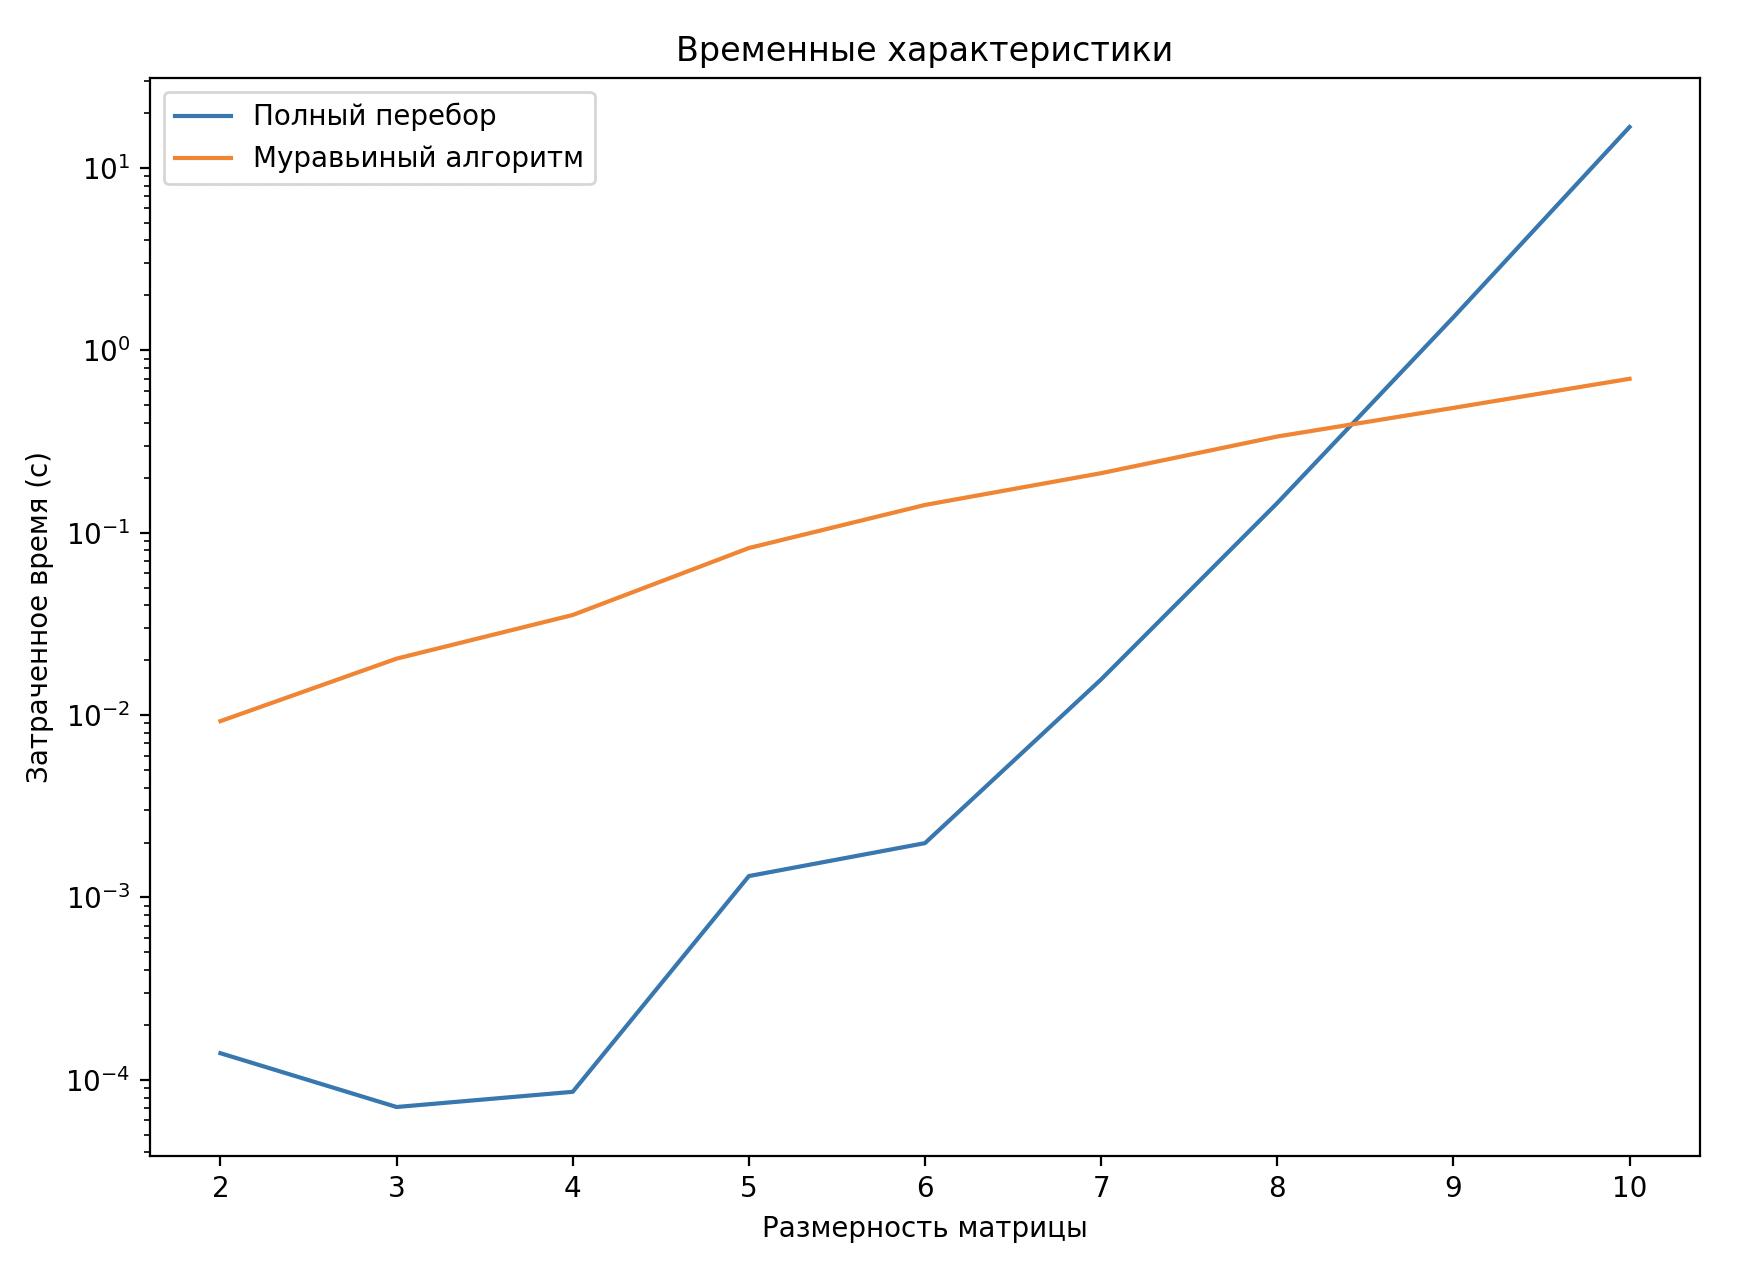
\includegraphics[height=0.50\textheight]{img/graph.png}
	\caption{График зависимости времени от размерности матрицы смежностей}
	\label{img:dem}
\end{figure}

\clearpage

Класс данных для параметризации представляет собой матрицу смежности с размерностью 9 \ref{matr:matrix}.

\begin{equation}
    \label{matr:matrix}
	K_{1} = \begin{pmatrix}
		0 & 9271 & 8511 & 2010 & 1983 & 7296 & 7289 & 3024 & 1011 \\
        9271 & 0 & 7731 & 4865 & 5494 & 6812 & 4755 & 7780 & 7641 \\
        8511 & 7731 & 0 & 1515 & 9297 & 7506 & 5781 & 5804 & 7334 \\
        2010 & 4865 & 1515 & 0 & 3662 & 9597 & 2876 & 8188 & 9227 \\
        1983 & 5494 & 9297 & 3662 & 0 & 8700 & 4754 & 7445 & 3834 \\
        7296 & 6812 & 7506 & 9597 & 8700 & 0 & 4216 & 5553 & 8215 \\
        7289 & 4755 & 5781 & 2876 & 4754 & 4216 & 0 & 4001 & 4715 \\
        3024 & 7780 & 5804 & 8188 & 7445 & 5553 & 4001 & 0 & 9522 \\
        1011 & 7641 & 7334 & 9227 & 3834 & 8215 & 4715 & 9522 & 0 
	\end{pmatrix}
\end{equation}

Для данного класса данных приведена таблица с выборкой 
параметров, которые наилучшим образом решают поставленную задачу.

\begin{table}[!ht]
    \centering
    \caption{\label{tab:par} Параметры для класса данных $K_{1}$}
    \begin{tabular}{|r|r|r|r|r|}
    \hline
        Альфа & Бетта & Дней & Оптимальный & Ошибка  \\ \hline
        0.1 & 0.2 & 500 & 27523 & 0  \\ \hline
        0.1 & 0.4 & 300 & 27523 & 0  \\ \hline
        0.1 & 0.8 & 500 & 27523 & 0  \\ \hline
        0.2 & 0.3 & 500 & 27523 & 0  \\ \hline
        0.2 & 0.6 & 100 & 27523 & 0  \\ \hline
        0.2 & 0.8 & 50 & 27523 & 0  \\ \hline
        0.3 & 0.1 & 300 & 27523 & 0  \\ \hline
        0.3 & 0.4 & 500 & 27523 & 0  \\ \hline
        0.3 & 0.6 & 300 & 27523 & 0  \\ \hline
        0.3 & 0.6 & 500 & 27523 & 0  \\ \hline
        0.3 & 0.7 & 500 & 27523 & 0  \\ \hline
        0.3 & 0.8 & 50 & 27523 & 0  \\ \hline
        0.3 & 0.8 & 500 & 27523 & 0  \\ \hline
        0.4 & 0.1 & 300 & 27523 & 0  \\ \hline
        0.4 & 0.5 & 300 & 27523 & 0  \\ \hline
        0.5 & 0.1 & 500 & 27523 & 0  \\ \hline
        0.5 & 0.2 & 300 & 27523 & 0  \\ \hline
        0.5 & 0.4 & 500 & 27523 & 0  \\ \hline
        0.5 & 0.5 & 300 & 27523 & 0  \\ \hline
    \end{tabular}
\end{table}

\section{Сравнение алгоритмов}
В таблице \ref{tab:sravn} представлен сравнительный анализ алгоримта полного перебора
и муравьиного перебора.

\begin{table}[!ht]
    \centering
    \caption{\label{tab:sravn} Сравнение алгоритма полного перебора с муравьиным алгоритмом}
    \begin{tabular}{|l|l|c|}
    \hline
        Методы / Критерии & Точность решения & Трудоемкость \\ \hline
        
        Метод полного пере-& Гарантирует & O(n!) \\
        бора & ~ & ~ \\ \hline

        Муравьиный алго-& Не гарантирует, так как присут-& $3n^2+n^4+$\\ 
        ритм & ствует случайный выбор началь-& $+m(3n+n^2*$ \\
        ~ & ного маршрута и вероятностный& $*(n^2+n^3))$ \\
        ~ & выбор в процессе работы. & ~ \\ 
        ~ & ~ & ~ \\ \hline
    \end{tabular}
\end{table}

\section{Вывод}

По результатам проделанных экспериментов можно сделать следующие выводы:
\begin{enumerate}[left=\parindent]
    \item при количестве вершин в графе до 8 алгоритм полного перебора работает
        быстрее муравьного алгоритма;
    \item при количестве вершин в графе более 8 время выполнения алгоритма
        полного перебора резко возрастает, в то время как у муравьиного
        алгоритма при переходе на следующее количество вершин время возрастает
        не более чем в 1.5 раза;
    \item лучшие результаты работы муравьиного алгоритма налюдались на парах значений:
        \begin{itemize}
            \item $\alpha = 0.1, \beta = 0.2, 0.4, 0.8$;
            \item $\alpha = 0.2, \beta = 0.3, 0.6, 0.8$;
            \item $\alpha = 0.3, \beta = 0.1, 0.4, 0.6, 0.7, 0.8$;
            \item $\alpha = 0.4, \beta = 0.1, 0.5$;
            \item $\alpha = 0.5, \beta = 0.1, 0.2, 0.4, 0.5$.
        \end{itemize} 
\end{enumerate}

